%!TEX root = ../../../adrien_gomar_phd.tex

In this thesis, only the front rotor blades vibration
and the flutter phenomenon are considered.

\subsection{Modes considered}
\label{sub:dream_ls_modes_considered}

Two structural modes are considered for the aeroelastic study of this 
configuration: the second bending/flexion mode and the first torsion mode
of the front rotor.
The shape of the modes is shown in Fig.~\ref{fig:dream_ls_ael_modes}.
Two inflection lines are seen for the 2F mode, hence its designation.
\begin{figure}[htb]
  \centering
  \subfigure[2F]{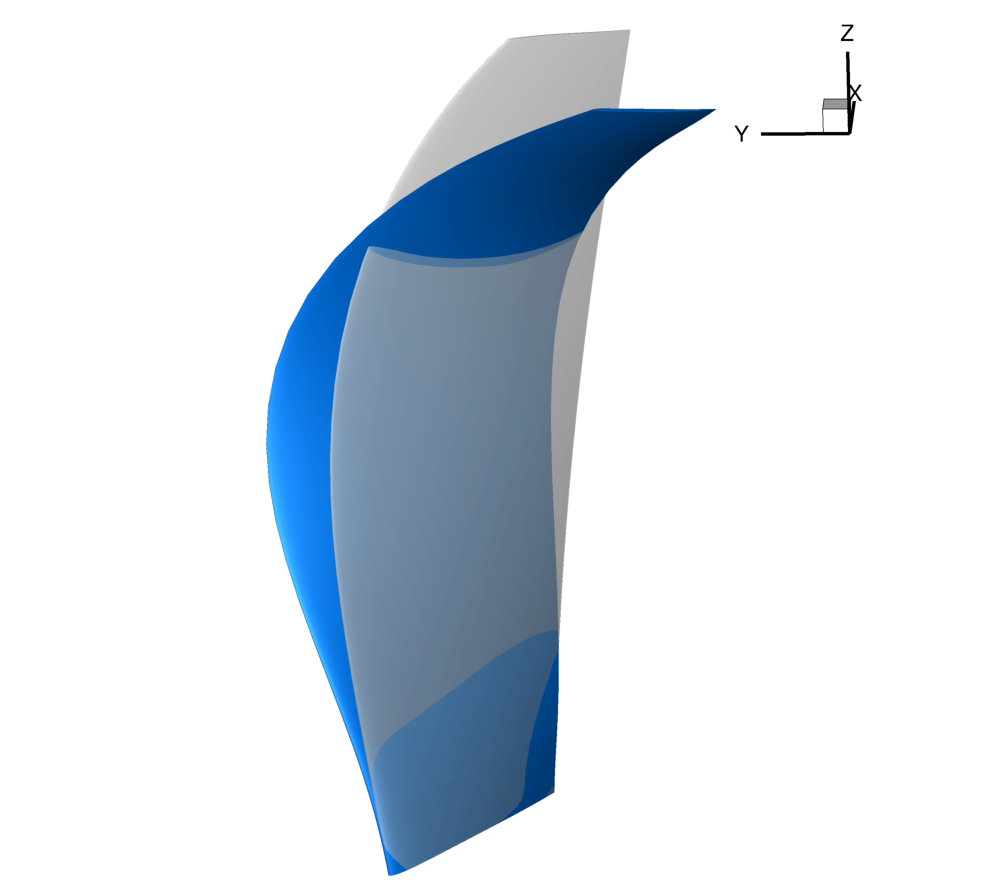
\includegraphics[height=.35\textwidth]{mode_2F.png}}
  \subfigure[1T]{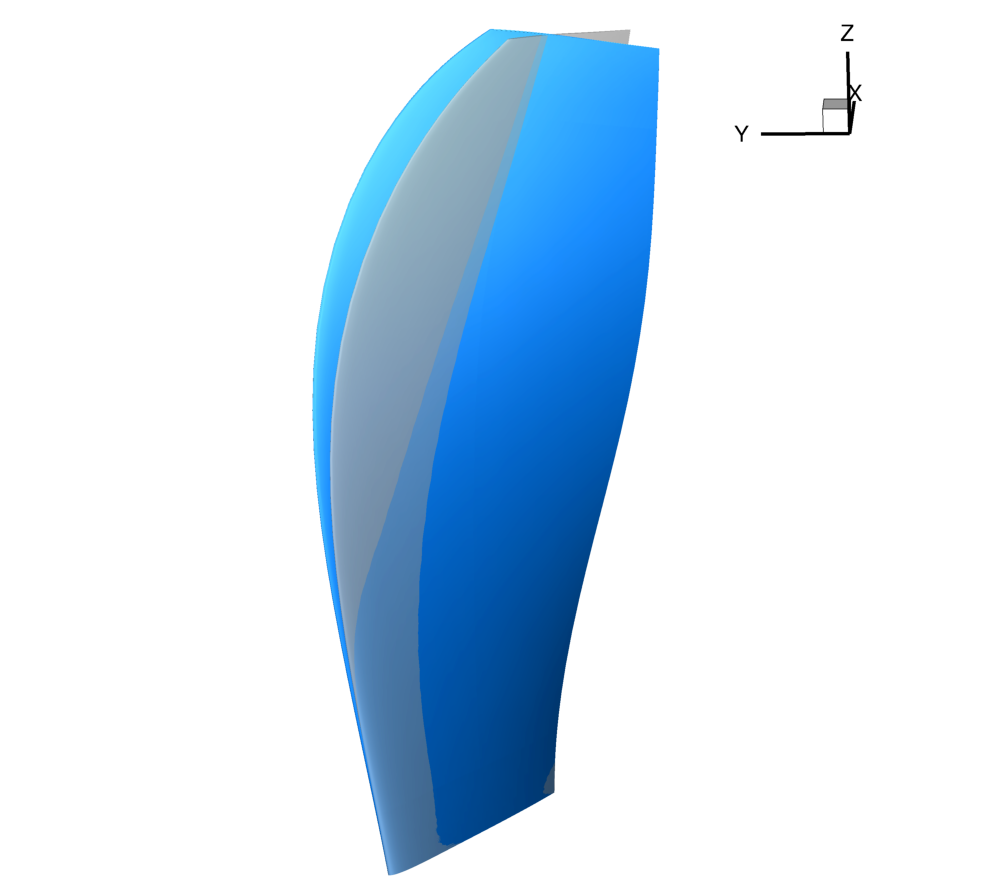
\includegraphics[height=.35\textwidth]{mode_1T.png}}
  \caption{Low-speed isolated configuration: structural modes considered.}
  \label{fig:dream_ls_ael_modes}
\end{figure}

As detailed in Chapter~\ref{cha:ael}, the modes have been identified
by using a structural code and were an input of the current thesis.
The \emph{elsA} solver is used (see Appendix~\ref{app:elsa}), along
with its aeroelastic module (AEL).
